\begin{figure}
    \begin{center}
        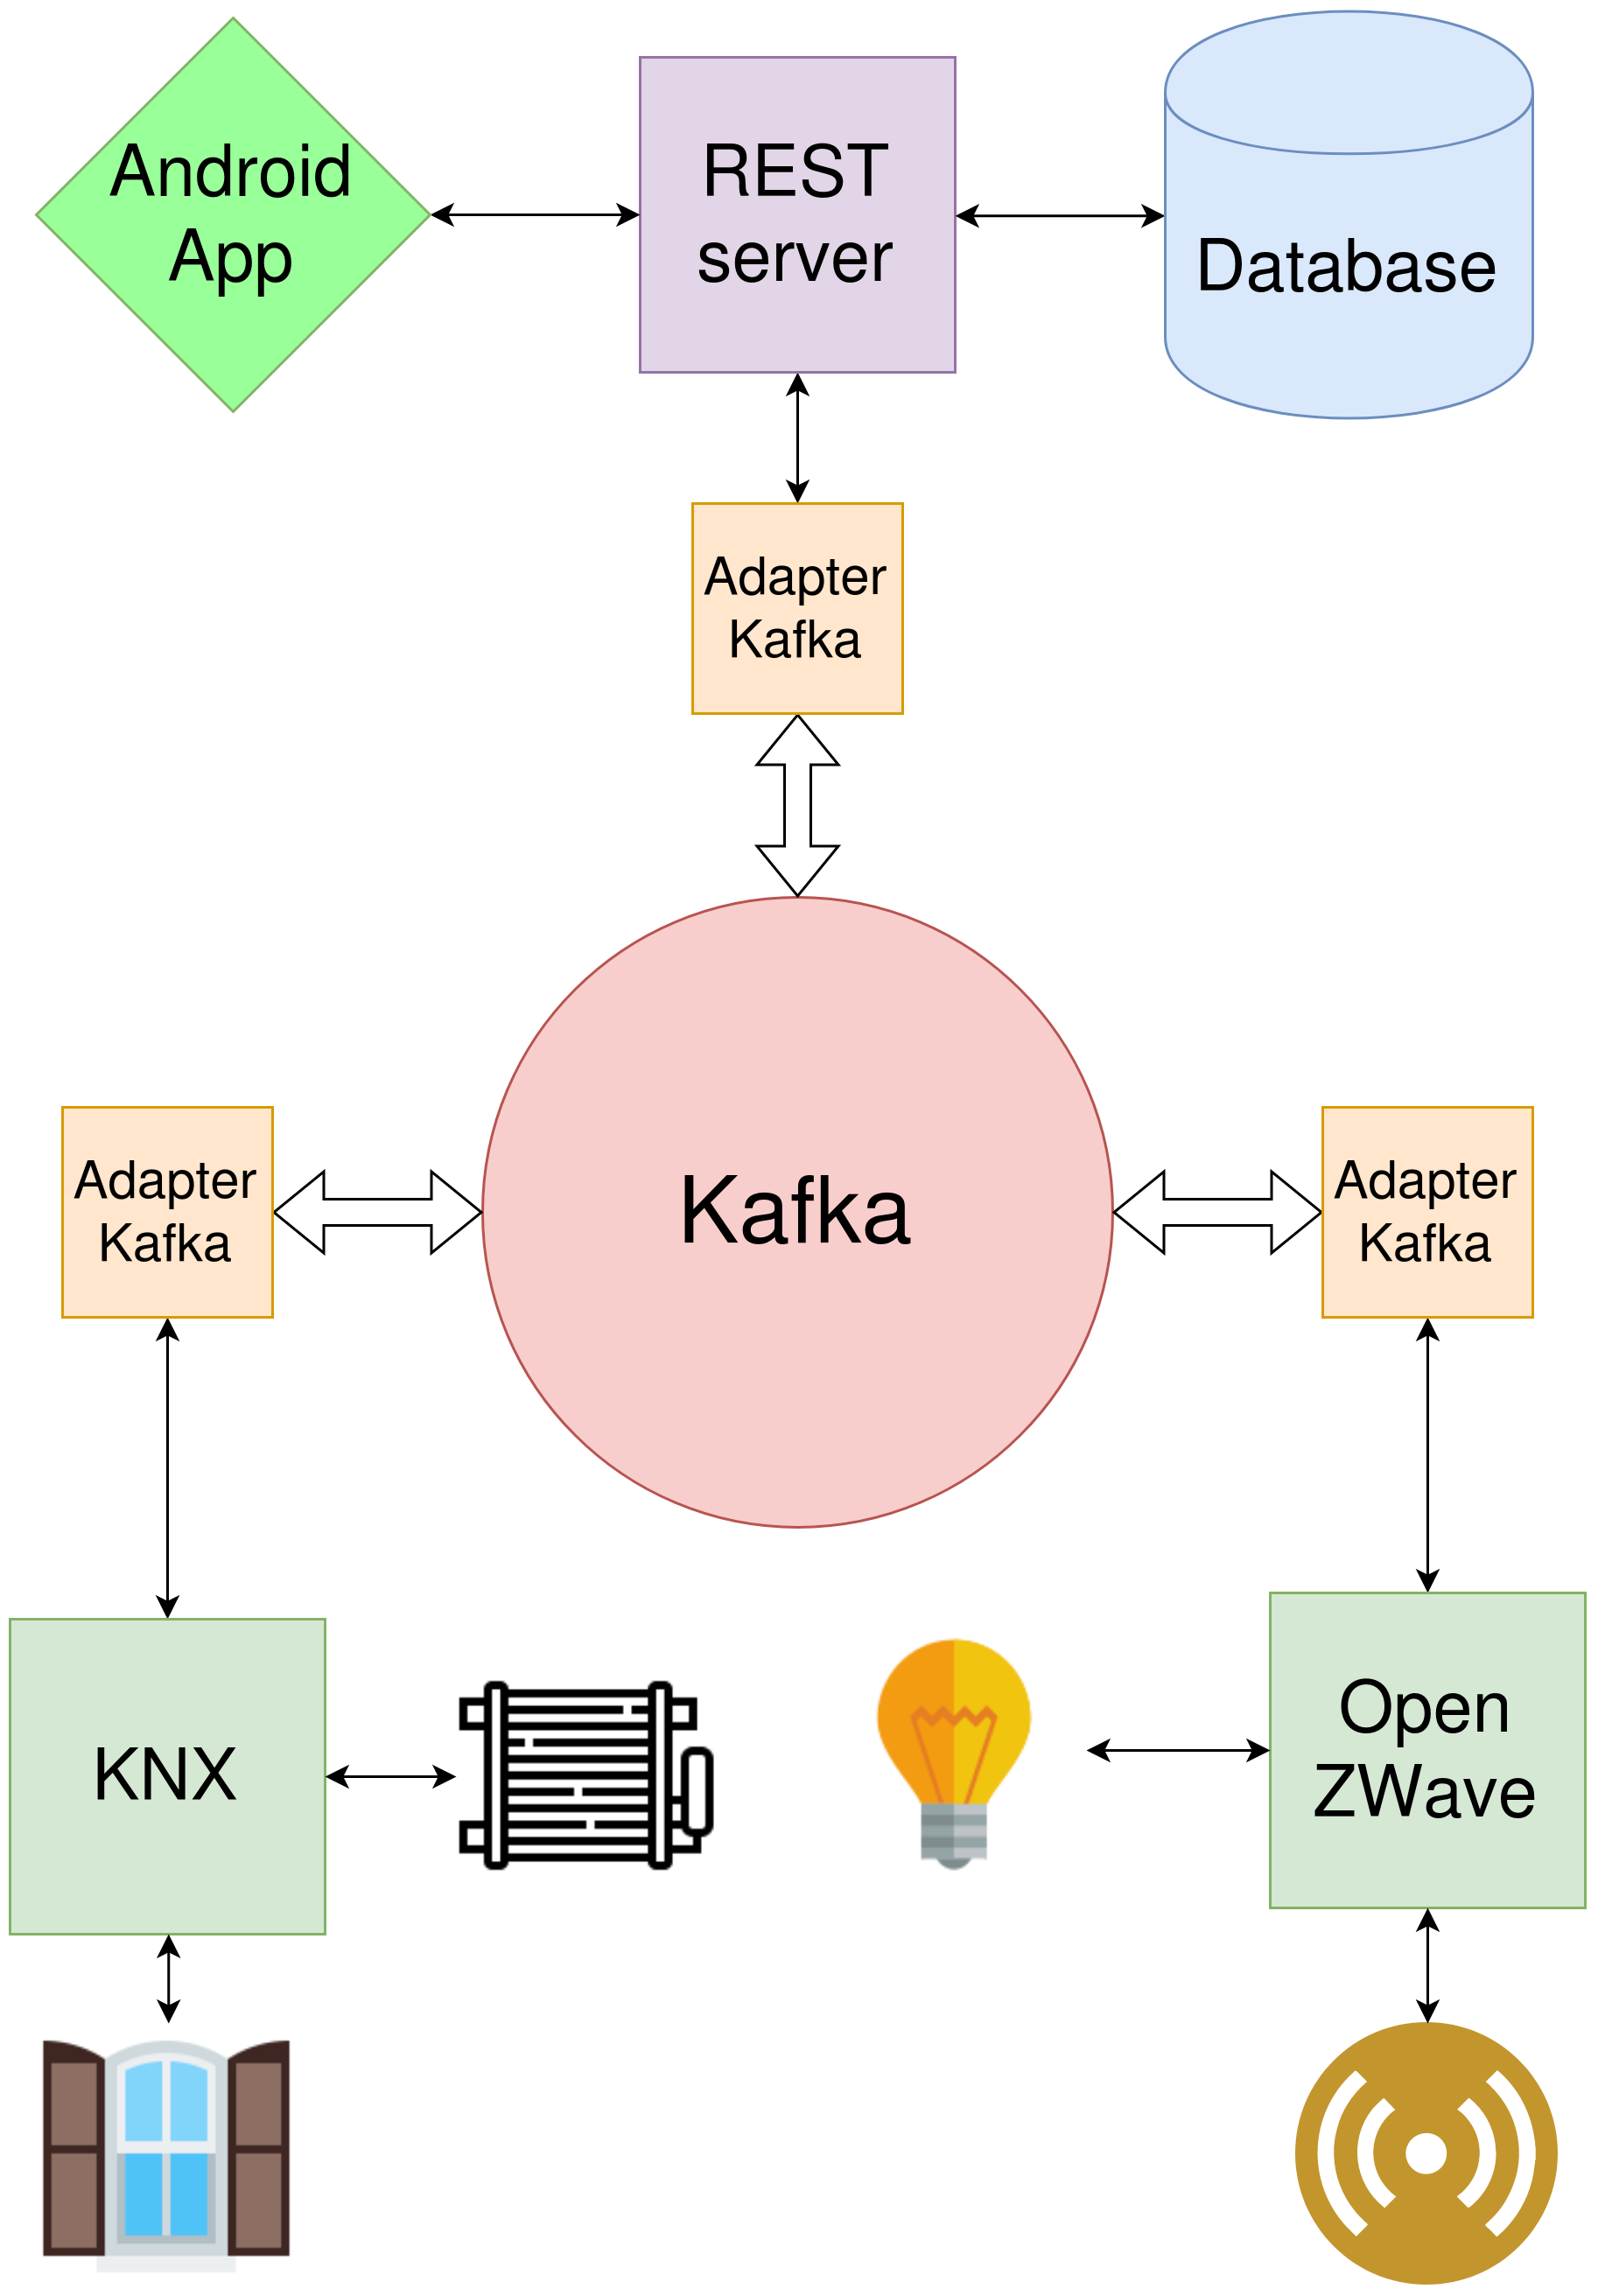
\includegraphics[width=0.8\textwidth]{img/general.png}
    \end{center}
    \caption{Architecture globale du système}
    \label{shema_general}
\end{figure}


\subsection{Protocole d'échange des messages}
Le Protocole d'échange des messages à été défini selon l'arcitecture visible à la figure "Architecture globale du système", les entités principales de l'application sont le client mobile, les devices KNS, les devices Openzwave et la base de données. Afin de tout mettre le tout en relation, nous avons procédé de manière à échanger les messages dans différents "topics" qui permettent d'identifier le sujet des messages.

\subsection{Statistiques}
En ce qui concernet les Statistiques, notre architecture de la base de données est pensée de manière à stocker les informations des différents devices dans le temps afin de pouvoir retraçer leurs parcours et établir les statistiques qui en découlent.